\chapter{Machine and Deep Learning in DNA sequence classification} \label{sec:dna_sequences}

\section{DNA sequences} \label{subsec:what_are_dna_sequences}

\gls{DNA} is composed of a linear string of nucleotides, or bases, which are referred to by their chemical names' first letters: \gls{A}, \gls{T}, \gls{C}, and \gls{G}. 

\gls{DNA} sequencing is the technique of finding the order of the four bases. Scientists can determine the type of genetic information carried in a \gls{DNA} segment by examining the sequence. Furthermore, and more significantly, sequencing data can reveal mutations in a gene that could lead to illness, by comparing a healthy and a mutated sequence~\cite{2020DNASheet}.

The four chemical bases of the \gls{DNA} double helix always connect with the same partner to produce "base pairs". \gls{A} is always paired with \gls{T}, while \gls{C} is always paired with \gls{G} (Figure~\ref{fig:dna}). This pairing explains the technique by which \gls{DNA} molecules are copied when cells divide, as well as the methods used in most \gls{DNA} sequencing research. The human \gls{genome} is made up of around 3 billion base pairs, which carry the instructions for creating and maintaining a human person~\cite{2020DNASheet}.

\begin{figure}[htbp]
    \centering
    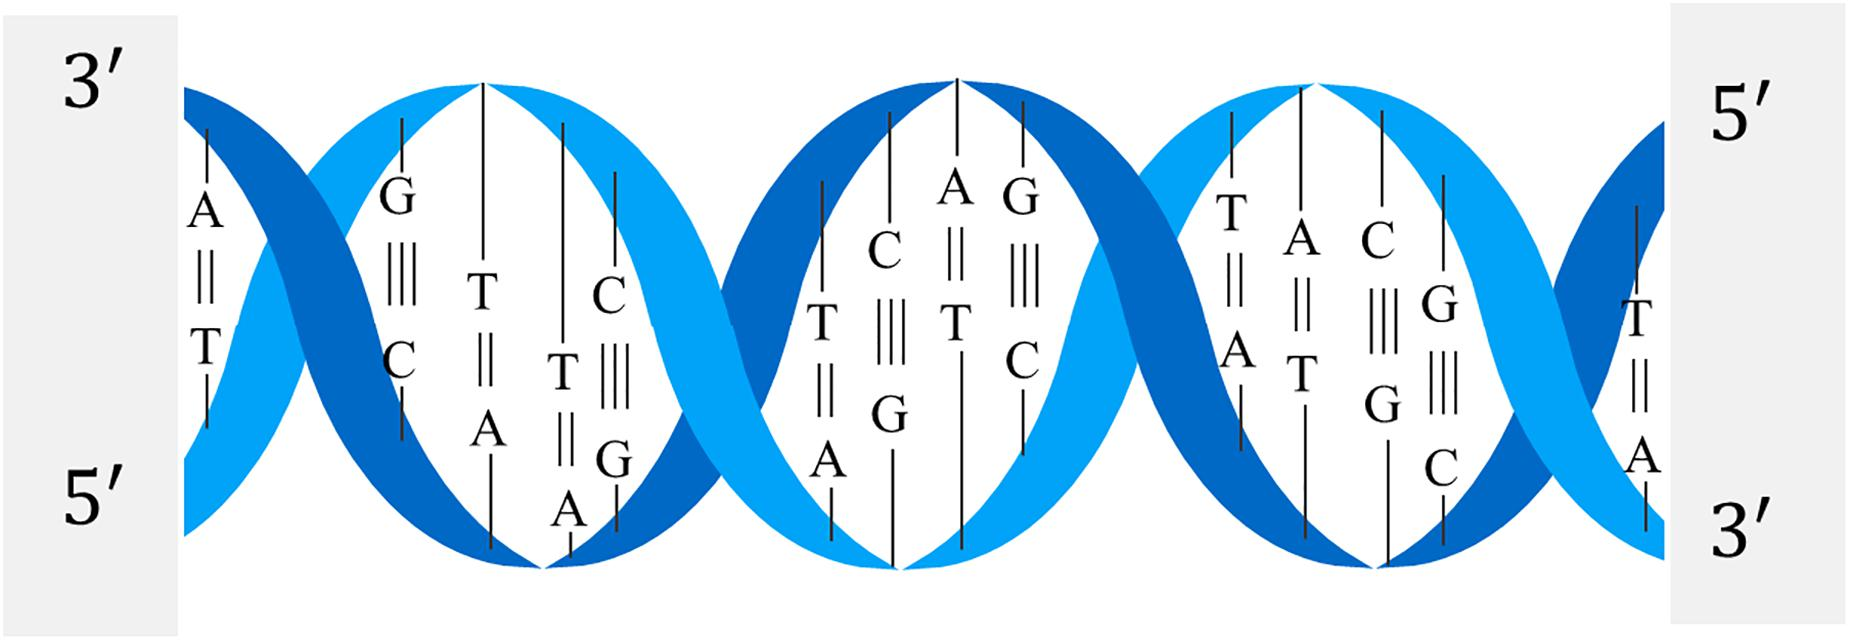
\includegraphics[width=0.5\linewidth]{Chapters/Figures/dna.jpg}
    \caption{Double helix of DNA~\cite{Yang2020ReviewDNA}}
    \label{fig:dna}
\end{figure}

Since the Human Genome Project's completion~\cite{TheProject}, technological advancements and automation have made it possible for individual genes to be sequenced on a regular basis, by reducing the amount of time it takes to perform the sequencing and also reducing its cost. Some labs can sequence over 100,000 billion bases per year, and a few thousand dollars is enough to sequence an entire \gls{genome}~\cite{2020DNASheet}. 

\section{DNA sequence classification - Traditional ML}

Understanding the connections between protein structure and function is one of Biology's main goals. The basic amino acid sequences provide particularly helpful structural information for understanding the structure-function paradigm. The idea that sequences with similar structures have comparable functions is used to classify \gls{DNA} sequences. Sequence alignment techniques such as BLAST~\cite{Altschul1990BasicTool} and FASTA~\cite{Pearson1988ImprovedComparison} have historically been used to determine sequence similarity, and the majority of sequence classification is still done by these methods. This decision is based on two primary assumptions: the functional components have similar sequence properties, and the functional elements' relative order is preserved across sequences. These assumptions are applicable in a wide range of situations, but they are not universal~\cite{LoBosco2017DeepClassification}.

Regardless, despite recent advancements, the major issue that severely restricts the use of alignment techniques remains their computational time complexity. As a result, many effective and computationally affordable approaches for analyzing sequence data have recently been presented. Since the majority of sequence analysis tasks are expressed as binary or multiclass classification tasks, \gls{ML} techniques have been playing an important role~\cite{Liu2017BioSeq-Analysis:Approaches}.

In \gls{ML}, the goal of classification is to use the training set to create a classification model that can predict the category of unknown incoming samples. \gls{DNA} sequence classification is the process of predicting the kind of \gls{DNA} sequence based on structural or functional similarities, then predicting the sequence function and relationships with other sequences, and finally assisting in the identification of genes in \gls{DNA} molecules~\cite{Yang2020ReviewDNA}.

However, for a \gls{ML} model to be able to predict, it first needs input features, and that is the main problem with sequences. The most difficult component is the feature selection because the sequences only consist of a set of four letters, meaning they lack explicit features. Converting sequences into an effective numerical representation that reflects the underlying relationship with the feature to be predicted can have a big impact on the model's performance~\cite{LoBosco2017DeepClassification,Chen2019ILearn:Data}.

It is standard practice to encode molecular information as numerical features in order to apply various \gls{ML} algorithms to molecular data. Molecular descriptors are one of the most powerful tools for describing the biological, physical, and chemical features of molecules, and they have been utilized in a variety of research to better understand molecular interactions. These descriptors capture and amplify different features of molecular topology in order to better understand how molecular structure influences molecular properties~\cite{Dong2018PyBioMed:Interactions}. However, it is worth emphasizing that these descriptors need to be manually created, meaning the feature selection is a handcrafted process. Some examples of \gls{DNA} sequence descriptors are the nucleic acid composition, structure composition and sequence length~\cite{Liu2017BioSeq-Analysis:Approaches,Chen2019ILearn:Data,Bonidia2021MathFeature:Descriptors}. Table~\ref{tab:descriptors_DNA} provides an overview of packages capable of calculating descriptors for not only \gls{DNA} but also \gls{RNA} and protein sequences. In addition, some of these packages also perform \gls{ML} functions on the calculated features.

\begin{table}[ht]
	\caption{Overview of packages with DNA descriptors}
	\label{tab:descriptors_DNA}
\centering
\begin{tabular}{lp{2cm}p{3.5cm}p{7cm}}
	\toprule
	\textbf{Year} & \textbf{Authors} & \textbf{Title} & \textbf{Focus}\\
	\midrule
	
	\citeyear{Liu2014RepDNA:Effects} & \citeauthor{Liu2014RepDNA:Effects} & repDNA~\cite{Liu2014RepDNA:Effects} & Generate widely used features reflecting the physicochemical properties and sequence-order effects of \gls{DNA}s and nucleotides \\\midrule
	
	\citeyear{Dong2016BioTriangle:Interactions} & \citeauthor{Dong2016BioTriangle:Interactions} & BioTriangle~\cite{Dong2016BioTriangle:Interactions} & Full pipelining from getting molecular data, molecular representation to constructing \gls{ML} models on \gls{DNA}, \gls{RNA} and protein sequences. \\\midrule
	
	\citeyear{Liu2017BioSeq-Analysis:Approaches} & \citeauthor{Liu2017BioSeq-Analysis:Approaches} & BioSeq-Analysis~\cite{Liu2017BioSeq-Analysis:Approaches} & Automatically completing feature extraction, predictor construction, and performance evaluation on \gls{DNA}, \gls{RNA} and protein sequences. \\\midrule
	
	\citeyear{Dong2018PyBioMed:Interactions} & \citeauthor{Dong2018PyBioMed:Interactions} & PyBioMed~\cite{Dong2018PyBioMed:Interactions} & Calculate numerous features of biological molecules, with the goal of constructing integrated analytical pipelines from data gathering, data validation, and descriptor calculation to modeling. \\\midrule
	
	\citeyear{Nikam2019Seq2Feature:Tool} & \citeauthor{Nikam2019Seq2Feature:Tool} & Seq2Feature~\cite{Nikam2019Seq2Feature:Tool} & Extract protein and \gls{DNA} sequence-based features \\\midrule
	
	\citeyear{Muhammod2019PyFeat:Sequences} & \citeauthor{Muhammod2019PyFeat:Sequences} & PyFeat~\cite{Muhammod2019PyFeat:Sequences} & Extract features from proteins, \gls{DNA}s and \gls{RNA}s, with a particular emphasis on features that capture information on the interaction of nearby residues. \\\midrule
	
	\citeyear{Chen2019ILearn:Data} & \citeauthor{Chen2019ILearn:Data} & iLearn~\cite{Chen2019ILearn:Data} & Feature extraction, clustering, normalization, selection, dimensionality reduction, predictor construction, best descriptor/model selection, ensemble learning and results visualization for \gls{DNA}, \gls{RNA} and protein sequences.\\\midrule
	
	\citeyear{Bonidia2021MathFeature:Descriptors} & \citeauthor{Bonidia2021MathFeature:Descriptors} & MathFeature~\cite{Bonidia2021MathFeature:Descriptors} & Implements mathematical descriptors able to extract relevant numerical information from \gls{DNA}, \gls{RNA} and proteins.\\
    
	\bottomrule
\end{tabular}
\end{table}

Another important stage in sequence analysis is the creation of predictors. Many \gls{ML} methods have been employed to predict structural and functional characteristics and to help in the annotation of genomic data. \gls{SVM}, \gls{RF}, \gls{ANN}, \gls{KNN}, and \gls{LgR} are some examples of these methods~\cite{Chen2019ILearn:Data}.


%Descriptors 
%Algorithms  

\section{DNA sequence classification - DL}

A common difficulty in data mining is classifying biological sequences as a specific data type. This is a tough challenge, due to the non-numerical properties of biological sequence elements, the sequence interaction between sequence elements, and the variable sequence length~\cite{Yang2020ReviewDNA}. \gls{ML} methods for supervised classification tasks are, without a doubt, heavily reliant on the feature selection stage, and it is required to detect and quantify relevant aspects of the objects to classify in order to develop a suitable representation. \gls{DL} models have recently been shown to be capable of automatically extracting meaningful features from input patterns~\cite{LoBosco2017DeepClassification}. This is possible due to feature learning techniques that \gls{DL} methods possess. These techniques allow the automatic identification of the representations required for feature detection from raw data, meaning that the human feature engineering is removed, and the machine will learn the features instead. As a result, \gls{DL} models only need the sequence itself as input, unlike \gls{ML} models that require the previously calculated features. However, first it is required to transform the string sequence into a numerical value in order to create an input matrix for the model~\cite{Yang2020ReviewDNA}. Sequential encoding, one-hot encoding, and k-mer encoding are three popular methods for sequence encoding~\cite{Choong2017EvaluationMethod} and Table~\ref{tab:encoding_methods} summarizes the differences between them. The encoding technique is also significant for classification accuracy.

\begin{table}[ht]
	\caption{DNA sequence encoding methods~\cite{Yang2020ReviewDNA}}
	\label{tab:encoding_methods}
\centering
\begin{tabular}{lp{8cm}}
	\toprule
	\textbf{Encoding Method} & \textbf{Features} \\
	\midrule
	
	Sequential encoding & Each base is encoded as a number. For example, change [A,T,G,C] to [0.25,0.5,0.75,1.0], and any other character to 0.\\\midrule
	
    One-hot encoding & Each base is encoded as a vector. [A,T,G,C] will become [0,0,0,1],[0,0,1,0],[0,1,0,0],[1,0,0,0]. These vectors can be combined into a 2-dimensional array.\\\midrule
    
    K-mer encoding & Decomposes a sequence into k-length overlapping segments. "ATGCATCGA" becomes "ATGCAT", "TGCATG", "GCATGC", "CATGCA"  when \textit{k}=6 is used. The segments must then be converted to numerical values.\\
    
	\bottomrule
\end{tabular}
\end{table}

In the case of the k-mer encoding method, the encoded sequence is not yet ready to be fed into the model, as the result of the encoding method is not a numerical value. The \gls{DL} model still needs this produced k-mer sentence to be transformed into a dense feature vector matrix and this can be achieved by using a word embedding layer. Word embedding is a technique for assigning each word in a sequence a continuous vector representation, and words with similar meanings are near in distance in the vector space generated.~\citeauthor{Gunasekaran2021AnalysisModels}~\cite{Gunasekaran2021AnalysisModels} used the k-mer encoding to generate segments of \gls{DNA} sequences and then applied the word embedding layer to their model to transform the sentence into a dense feature vector matrix. It is also possible to apply an embedding layer to other encoding methods. Although there is no semantic similarity to uncover, this concept has also been applied at character-level, representing a first step toward completely automated feature learning. For example,~\citeauthor{LoBosco2017DeepClassification}~\cite{LoBosco2017DeepClassification} used \gls{CNN} and \gls{RNN} for the purpose of \gls{DNA} sequence classification. For both models, their first layer was an embedding layer, which accepted as input 16-dimensional one-hot encoding of sequence characters and produced a 10 dimensional continuous vector. The embedding representation may be achieved using a single feed-forward layer using random weights in order to learn embedding for all of the terms in the training dataset.

In Section~\ref{sec:previous_work}, relevant previous work on DNA classification will be provided, and it is possible to conclude that \gls{CNN} and \gls{RNN} are the most commonly used \gls{DL} models.

\section{Relevant previous work on DNA classification}\label{sec:previous_work}

\gls{DNA} sequence classification is a critical problem in biomedical research, and since current solutions involve the use of homologies, which is a long and costly process, multiple \gls{ML} techniques were used to successfully complete this task. In recent years, numerous articles and papers were published regarding this classification challenge with both traditional \gls{ML} and \gls{DL} approaches.

% [X]
\citeauthor{Nair2010ANNRepresentation}~\cite{Nair2010ANNRepresentation} proposed a unique technique for organism classification based on a combination of \gls{FCGR} and \gls{DNA}. \gls{CGR} displays \gls{DNA} sequences in a unique way and reveals hidden patterns in them. The frequency of sub-sequences contained in the \gls{DNA} sequence is shown by \gls{FCGR}, which is developed from \gls{CGR}. The taxonomic distribution of Eukaryotic species is broken down into eight groups, and \gls{ANN} is used to classify them.

% [X]
\citeauthor{Rizzo2015AClassification}~\cite{Rizzo2015AClassification} introduced a \gls{DNN} based on spectral sequence representation for \gls{DNA} sequence classification. The framework is evaluated on a dataset of 16S genes, and its results are compared to the General Regression Neural Network as well as Naive Bayes, \gls{RF}, and \gls{SVM} classifiers in terms of accuracy and F1 score. When it came to classifying short sequence fragments of 500 bp, the \gls{DL} technique beat all other classifiers.

% [X]
\citeauthor{Nguyen2016DNANetwork}~\cite{Nguyen2016DNANetwork} developed a new method for classifying \gls{DNA} sequences using a \gls{CNN} while treating them as text input. Because the authors employed one-hot vectors to represent sequences as input to the model, the important position information of each nucleotide in sequences is preserved. The authors investigated the suggested model using 12 \gls{DNA} sequence datasets and found substantial improvements in all of them. Out of the 12 datasets used, 10 of them include DNA sequences that wrap around histone proteins (for example, H3 and H4) and the other datasets are Splice and Promoter datasets. This finding suggests that a \gls{CNN} can be used to handle additional sequence challenges in bioinformatics.

% [X]
\citeauthor{LoBosco2017DeepClassification}~\cite{LoBosco2017DeepClassification} offer two distinct \gls{DL} architectures (\gls{CNN} and \gls{RNN}) for \gls{DNA} sequence classification. For five separate classification tasks, they compare their results using a public data set of \gls{DNA} sequences. Two \gls{DL} architectures were examined in this work for automated classification of bacteria species with no sequence preprocessing procedures. In comparison to a traditional \gls{CNN}, the authors have presented a \gls{LSTM} that utilizes the nucleotide locations in a sequence. The \gls{CNN}s outperform the \gls{LSTM} in the four easiest classification tasks, but their performance deteriorates in the last, when the \gls{LSTM} performs better. %character-level one-hot encoding

% [X]
\citeauthor{Abd-Alhalem2020BacterialLayers}~\cite{Abd-Alhalem2020BacterialLayers} proposed, based on a custom layer, a new technique for classification of bacterial \gls{DNA} sequences. The \gls{FCGR} of \gls{DNA} is employed with a \gls{CNN}. With a proper choice of the frequency k-lengthen words occurrence in \gls{DNA} sequences, the \gls{FCGR} is used as a sequence representation technique. The \gls{DNA} sequence is mapped using \gls{FCGR}, which generates a gene sequence image. Both local and global patterns may be seen in this sequence. For image classification, a pre-trained \gls{CNN} is used. 

% [X]
\citeauthor{Chen2017AClassification}~\cite{Chen2017AClassification} explain the distinction between cell-free DNA and normal DNA. The authors employed a variety of classification models to categorize normal and cfDNA, including \gls{KNN}, \gls{SVM}, and \gls{RF}. In comparison to all other algorithms, the authors determined that the \gls{RF} had the best accuracy. %DNA fragmentation patterns

\citeauthor{Shen2018RecurrentSites}~\cite{Shen2018RecurrentSites} introduced a model that combines a Bidirectional \gls{GRU} network with k-mer embedding to discover \gls{TF} binding sites on \gls{DNA} sequences. \gls{DNA} sequences are split into k-mer sequences of varying lengths and stride windows. Then, they take each k-mer as a word and train a word representation model on it using the \textit{node2vec} technique. With this technique, the vectors are carefully designed in such a way that a simple mathematical function reflects the amount of semantic similarity between the words represented by those vectors. This means that words with common contexts are placed close to one another in the vector. Finally, for feature learning and classification, they built a deep bidirectional \gls{GRU} model.

% [X]
\citeauthor{Helaly2019ConvolutionalStudy}~\cite{Helaly2019ConvolutionalStudy} analyze three of the most current \gls{DL} efforts for taxonomy classification using the 16S rRNA barcode dataset. Three distinct \gls{CNN} architectures are examined, as well as three different feature representations: k-mer spectral representation, \gls{FCGR}, and character-level integer encoding. The most fine-grained classification challenge showed that representations that hold positional information about the nucleotides in a sequence perform substantially better.

%%%%%%%%%%%%%%%%%%%%%%%%%%%%%%%%%%%%%%%%%%%%%%%%%%%%%%%%%%%%%%%%%%%%%%
%\citeauthor{Zhang2020AData}~\cite{Zhang2020AData} asjdk

\citeauthor{Zhang2020DeepHE:Learning}~\cite{Zhang2020DeepHE:Learning} proposed a \gls{DL} based technique (fully connected \gls{DNN}) for predicting human essential genes by combining features acquired from sequencing data with a protein-protein interaction network. An embedding method (\textit{word2vec}) is used to automatically learn the features, as well as 89 sequence features derived from \gls{DNA} sequence and protein sequence for each gene. They outperform numerous traditional \gls{ML} models, such as \gls{SVM}, Naïve Bayes, \gls{RF}, and Adaboost, using the same features. Results show that the final model can accurately predict human gene essentiality with an average performance of AUC higher than 94\%.

%%%%%%%%%%%%%%%%%%%%%%%%%%%%%%%%%%%%%%%%%%%%%%%%%%%%%%%%%%%%%%%%%%%%%%

% [X]
\citeauthor{Gunasekaran2021AnalysisModels}~\cite{Gunasekaran2021AnalysisModels} used \gls{CNN}, \gls{CNN}-\gls{LSTM}, and \gls{CNN}-Bidirectional \gls{LSTM} architectures with Label and k-mer encoding for \gls{DNA} sequence classification. Different classification metrics were used to evaluate the models. According to the findings of the experiments, the \gls{CNN} and \gls{CNN}-Bidirectional \gls{LSTM} with k-mer encoding have good accuracy, with 93.16\% and 93.13\% on testing data, respectively.

% [X]
\citeauthor{Lugo2021AIdentification}~\cite{Lugo2021AIdentification} presented a sequential \gls{DL} approach for bacterium identification. To derive an identification model for whole-genome bacterium sequences, the proposed neural network takes advantage of the massive volumes of data supplied by Next-Generation Sequencing. The bidirectional \gls{RNN} (BI-\gls{GRU}) outperformed other classification algorithms (Naive Bayes, Multilayer Perceptron) after verifying the identification model. In a low-dimensional space, a distributed representation was proven as the appropriate encoding for bacterial genetic information. The distributed representation is given context by combining two or more k-mer lengths. Context makes use of positional data, which is critical in biological sequences.

Table~\ref{tab:previous_work} provides an overview of the previous work on DNA classification described above.

%%%%%%%%%%%%%%%%%%%%%%%%%%%%%%%%%%%%%%%%%%%%%%%%%%%%%%%%%%%%%%%%%%%%%%%%%%%%%%%%%%%%%%%%%%%%

\begin{footnotesize}
\begin{longtable}{lp{1.5cm}p{3.3cm}p{3cm}p{2.2cm}p{2.7cm}}
    \caption{Overview of DNA classification's previous work}
	\label{tab:previous_work}
	\endfirsthead
    \endhead
	\toprule
	\textbf{Year} & \textbf{Authors} & \textbf{Title} & \textbf{Focus} & \textbf{Classifier} & \textbf{Features / Encoding}\\
	\midrule
	
	\citeyear{Nair2010ANNRepresentation} & \citeauthor{Nair2010ANNRepresentation} & \citetitle{Nair2010ANNRepresentation}~\cite{Nair2010ANNRepresentation} & Taxonomic classification of Eukaryotic species & \gls{ANN} & FCGR\\\midrule
	
	\citeyear{Rizzo2015AClassification} & \citeauthor{Rizzo2015AClassification} & \citetitle{Rizzo2015AClassification}~\cite{Rizzo2015AClassification} & Classify 16S bacterial genomic sequences & \gls{DNN}, General Regression Neural Network, Naive Bayes, \gls{RF}, \gls{SVM} & k-mer encoding\\\midrule
	
	\citeyear{Nguyen2016DNANetwork} & \citeauthor{Nguyen2016DNANetwork} & \citetitle{Nguyen2016DNANetwork}~\cite{Nguyen2016DNANetwork} & Solve DNA sequence classification problem in 12 datasets & \gls{CNN} & one-hot vectors\\\midrule
	
	\citeyear{LoBosco2017DeepClassification} & \citeauthor{LoBosco2017DeepClassification} & \citetitle{LoBosco2017DeepClassification}~\cite{LoBosco2017DeepClassification} & Classification of bacteria species with no steps of sequence preprocessing & \gls{CNN}, \gls{RNN} & Character-level one-hot encoding\\\midrule
	
	\citeyear{Chen2017AClassification} & \citeauthor{Chen2017AClassification} & \citetitle{Chen2017AClassification}~\cite{Chen2017AClassification} & Cell-free DNA and normal DNA classification & \gls{KNN}, \gls{SVM}, \gls{RF} & DNA fragmentation patterns\\\midrule
	
	\citeyear{Shen2018RecurrentSites} & \citeauthor{Shen2018RecurrentSites} & \citetitle{Shen2018RecurrentSites}~\cite{Helaly2019ConvolutionalStudy} & Identify and classify \gls{TF} binding sites on \gls{DNA} sequences. & BI-\gls{GRU} & k-mer, word2vec \\\midrule
	
	\citeyear{Helaly2019ConvolutionalStudy} & \citeauthor{Helaly2019ConvolutionalStudy} & \citetitle{Helaly2019ConvolutionalStudy}~\cite{Helaly2019ConvolutionalStudy} & 16S rRNA barcode dataset taxonomy classification & \gls{CNN} & k-mer spectral representation, \gls{FCGR}, and character-level integer encoding\\\midrule

    
    \citeyear{Zhang2020DeepHE:Learning} & \citeauthor{Zhang2020DeepHE:Learning} & \citetitle{Zhang2020DeepHE:Learning}~\cite{Zhang2020DeepHE:Learning} & Pedict human essential genes on \gls{DNA} sequences & fully connected \gls{DNN} & word2vec, sequence features derived from \gls{DNA} sequence and protein sequence\\\midrule
	
	\citeyear{Gunasekaran2021AnalysisModels} & \citeauthor{Gunasekaran2021AnalysisModels} & \citetitle{Gunasekaran2021AnalysisModels}~\cite{Gunasekaran2021AnalysisModels} & COVID, SARS, MERS, dengue, hepatitis, and influenza classification & \gls{CNN}, \gls{CNN}-\gls{LSTM}, \gls{CNN}-Bidirectional, \gls{LSTM} & Label and k-mer encoding\\\midrule
	
    \citeyear{Lugo2021AIdentification} & \citeauthor{Lugo2021AIdentification} & \citetitle{Lugo2021AIdentification}~\cite{Lugo2021AIdentification} & Bacterium identification & BI-\gls{GRU} & Distributed k-mer \\
    
	\bottomrule
    
\end{longtable}
\end{footnotesize}
